\chapter{\label{chap:evaluation}Evaluation}
We evaluated the viability of our DAO as a Big Tech alternative. An ideal evaluation would be by measuring the impact of a large-scale (millions of users) and long term deployment of MusicDAO in terms of artist income and artist happiness. However, the time and scale required is not feasible in the scope of this thesis. Instead, we deploy MusicDAO on a smaller scale (20 Android devices, 11 users). We measure performance of money transaction flow, music streaming and search latency in supervised and unsupervised experiments. These measurements determine the responsiveness of our infrastructure in small network sizes. By comparing latency and throughput in several network sizes, we can make conclusions of the performance of our infrastructure in larger networks.

In an \textit{unsupervised} experiment, all test subjects are given the MusicDAO application and are asked to stream music and send money to artists, but with no specific rules or guidelines. We have no control over the actions of these test subjects.

In multiple \textit{supervised} experiments, we use 10 Android devices that are under our control. we measure latency and throughput of music data and money transfers, and analyze the impact of network size on these measurements.

% Discuss influence of BEP42 in bittorrent DHT network, our seedbox nodes may be blacklisted or throtled by other DHT nodes because our seedboxes are seeding a large amount of torrents (100) while having only 1 static ipv4 address

\section{Unsupervised experiment: public release}
MusicDAO was released publicly on the Google Play store and 11 test subjects were given the task to download music and send donations to artists. Upon installation and first running MusicDAO, it sends a request in the background to our Bitcoin node, asking for 10 coins in starter money. The responsiveness of our Bitcoin node for transferring starter money is analyzed in \ref{starter-money-flow}.

\subsection{Automated starter money transactions}
\label{starter-money-flow}
We analyze the responsiveness of our bitcoin node by obtaining two datasets, and inspecting their correlation in terms of timing of events.

The two datasets are: 
\begin{enumerate}
    \item App installations per day, as measured by the Google Play console.
    \item Transactions from our Bitcoin node with a value of 10 coins, scraped from our blockchain.
\end{enumerate}

When there are $x$ app installations on some day, there should be $y \gte x$ transactions outgoing from our Bitcoin faucet. In the graph shown by \ref{fig:faucet-app-installs}, this is not always the case. On 19-01-2021 there was (at least) one transaction missing. This was due to a server outage where the Bitcoin faucet was running. There are also cases in which there are transactions but no installations. This may be due to multiple app installations from one device on the same day (which is measured as one by the Google Play store console) or app installations outside of the Play store. 
\begin{figure}
    \centering
    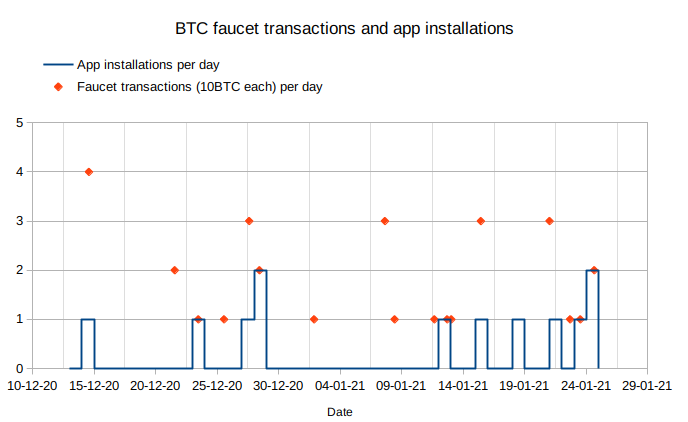
\includegraphics[width=0.7\textwidth]{evaluation/faucet-app-installs.png}
    \caption{Graph showing the relationship between faucet transactions of 10BTC and app installations. Every app installation should correspond to at least one faucet transaction.}
    \label{fig:faucet-app-installs}
\end{figure}

\subsection{Donation money flow}
The datasets used to create the plots shown in figs. \ref{fig:artist-income} and \ref{fig:transactions} are received by scraping blockchain block data from our Bitcoin node. Fig. \ref{fig:artist-income} shows the relation between created blocks and money transacted per block (cumulative). We observe that, during the timeline of the release experiment, nearly 500 BTC has been received by artists.

Note that the Bitcoin blockchain only contains timestamps for blocks, and no timestamps for individual transactions. This means we could not analyze transaction confirmation time in our unsupervised experiment, as this requires the timestamp of creating a transaction. However, prediction and analysis of confirmation times in Bitcoin have already been performed multiple times in recent literature~\citep{kawase2017transaction}~\citep{koops2018predicting}.
\begin{figure}
    \centering
    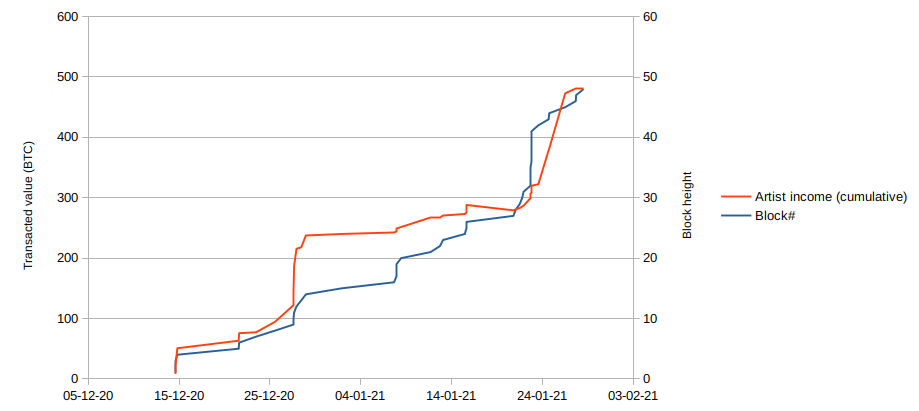
\includegraphics[width=0.9\textwidth]{evaluation/artist-income.png}
    \caption{Artist income (cumulative) over time and block creation}
    \label{fig:artist-income}
\end{figure}
We observe that artist income is 

\begin{figure}
    \centering
    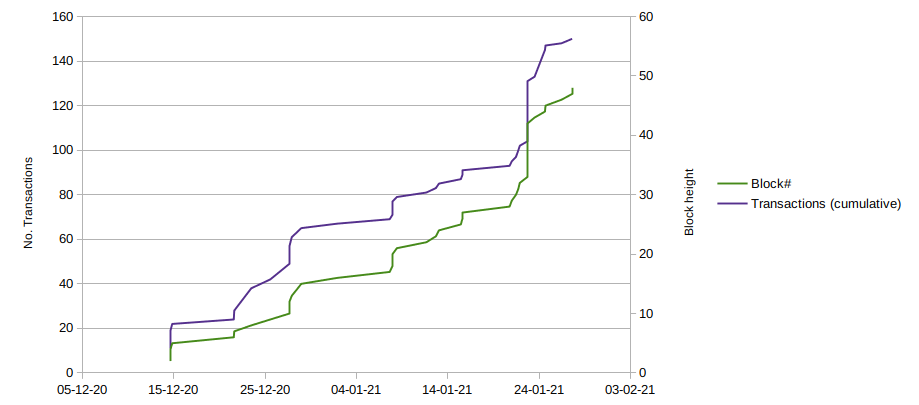
\includegraphics[width=0.9\textwidth]{evaluation/transactions.png}
    \caption{Transactions (cumulative) over time and block creation}
    \label{fig:transactions}
\end{figure}

\section{Supervised experiments}
During several supervised experiments, we were in control of a network of 10 Android devices, of which 5 virtual emulators and 5 real world devices. By performing several experiments, throughput and latency of several actions in this network is analyzed. Performing measurements in different network sizes (2 up to 10 devices), enables making predictions of the scalability of MusicDAO.

\subsection{Downloading and streaming}
\ref{fig:download-times} shows the download time of each stage in the bittorrent downloading process. By running 10 runs per network configuration, we inspected the effects of a bittorrent tracker on throughput and handshake time. The 4 different download stages marked in this figure are as follows.
\begin{enumerate}
    \item Time to receive metadata (including establishing handshake)
    \item Time to fill stream buffer
    \item Time to download first track
    \item Time to download full album
\end{enumerate}
\begin{figure}
    \centering
    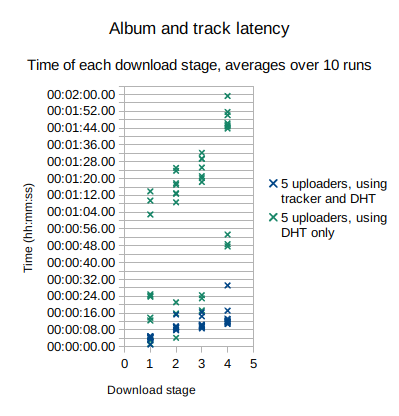
\includegraphics[width=0.5\textwidth]{evaluation/download-times.png}
    \caption{Average time spent per download stage. Measured by 20 runs in total, in two different network configurations.}
    \label{fig:download-times}
\end{figure}
The measurements show that a bittorrent tracker significantly reduces transfer times, for a small bittorrent swarm with 5 seeders. The largest difference is in the \textit{fetching metadata} stage, during which the device under test must find and connect with seeders. Discovering seeders over DHT requires asking multiple peers, and as such requires more time and messages before the download can start. Once the download starts, the runs using a tracker also reach significantly higher throughput, as the tracker assists the device in finding more seeders and healthier seeders. We found that the major factor slowing down download stages when using DHT only is the NAT puncturing stage, where devices try to connect to each other when there are one or more NAT devices in between. As expected, finding peers over DHT is also slower than via a tracker, however the time taken to create a handshake during NAT puncturing has a much larger effect on the peer-to-peer connecting time (the time taken to create a reliable connection for data transfer). 

\ref{fig:download-traces} shows 5 traces of downloading a 38 Megabyte album. The red line shows the moving average over these 5 runs. The slow-start nature of bittorrent can be observed here. Roughly the first 5 seconds are used for fetching the bittorrent metadata (see also \ref{fig:download-times}).
\begin{figure}
    The datasets used to create the plots shown in figs. \ref{fig:artist-income} and \ref{fig:transactions} are received by scraping blockchain block data from our Bitcoin node. Fig. \ref{fig:artist-income} shows the relation between created blocks and money transacted per block (cumulative). We observe that, during the timeline of the release experiment, nearly 500 BTC has been received by artists.

\centering
    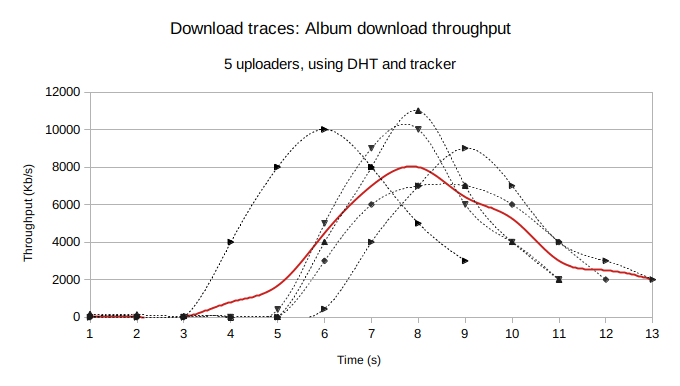
\includegraphics[width=0.7\textwidth]{evaluation/download-traces.png}
    \caption{5 traces of download throughput, downloading an album of around 38 Mbs. Measured with Nokia 7.}
    \label{fig:download-traces}
\end{figure}

Note that all devices evaluated in experiments \ref{fig:download-times} and \ref{fig:download-traces} use Bittorrent Local Peer Discovery. This means that some of the data transfers may be over local area network, which reaches considerably higher throughput than regular transfers. 

\subsection{Content discovery}
Fig. \ref{fig:content-discovery} shows measurements of an Android device discovering content, after running MusicDAO for the first time. More specifically, it is a measurement of music metadata, received as TrustChain blocks. All participating devices are configured as follows: Every device sends a random block to a random peer every 5 seconds. A Nokia 7 Android device ran the MusicDAO in an idle state for 5 minutes. The app measured the amount of content metadata discovered every 2 seconds. 

\subsubsection{\textbf{Mathematical model for evaluating experiment data}}
For evaluating content discovery over time, we compare three different experiments with a mathematical model for expected discovered items over time.
\begin{itemize}
    \item Gossip interval $i=5$ seconds
    \item Total items to discover: $R=50$
\end{itemize}
We device \textit{hit chance} as such: every interval $i$, the hit chance $C$ to receive any item is $$C=1-(\frac{p-1}{p})^p$$ with $p$ as the number of peers. This is according to \textit{Montmort's Matching Problem}~\citep{de1713essay}. We compute $C$ for the network sizes $n=2, n=4, n=10$ with $$p=n-1$$ The expected value for the cumulative amount of unique items discovered after $x$ iterations is $$E[R]=R(1-(\frac{R-1}{R})^{Cx})$$ where $$x=\frac{1}{i}$$ This expected value $E[R]$ over time is plotted in \ref{fig:content-discovery} as Model, for three different network sizes $n$.

\begin{figure}
    \centering
    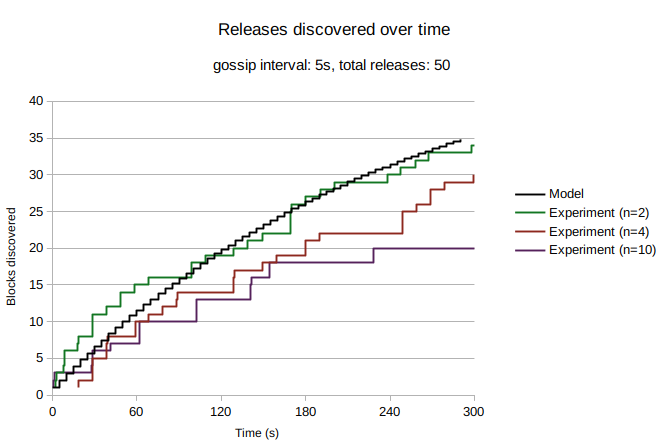
\includegraphics[width=0.8\textwidth]{evaluation/expected-vs-simulated-releases.png}
    \caption{Measurements of content discovery: releases discovered after a fresh installation. $n$: network size (amount of Android devices)}
    \label{fig:content-discovery}
\end{figure}
In \ref{fig:content-discovery} we can see a correlation between model and experiment for network sizes $n=2$ and $n=4$. For $n=10$ the experiment and model correlate until 3 minutes into the experiment. The reasons for this are for now not clear. More investigation and more experiments on larger networks are necessary to make conclusions.

\subsection{Random access latency}
Random access latency is evaluated through measuring search latency. Search latency is the round-trip time between initiating keyword search and receiving metadata for the release.  During this experiment, the content that was searched for was present in all devices except the one under test. The aforementioned distributed search algorithm (alg. \ref{alg:algorithm-distributed-search}) is used with the following parameters.
\begin{itemize}
    \item $maxPeers=20$
    \item $ttl=1$ 
\end{itemize}
This means that a maximum of 20 neighbours are contacted when performing a search, and that search is not recursive; meaning only neighbours are contacted (not neighbours of neighbours).

For two different situations, 10 runs are done and the latency and average latency are plotted in \ref{fig:search-latency}. We observe that for these 20 runs, latency is $<1s$. Another observation is: increase in network size (10 versus 2) does not negatively affect latency. Current music streaming systems have a search latency of roughly $<2s$ in ideal situations.

\begin{figure}
    \centering
    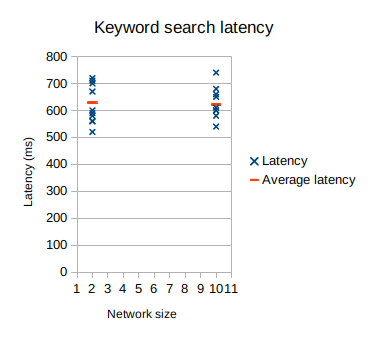
\includegraphics[width=0.5\textwidth]{evaluation/search-latency.png}
    \caption{Search latency of performing keyword search}
    \label{fig:search-latency}
\end{figure}

\section{Devices behind NATs}
During experimentation, some of the Bittorrent traffic on Android devices were blocked by Network Address  Translators (NATs). MP3 transfers over Bittorrent were slowed down by this. The NAT Port Mapping Protocol (NAT-PMP) was used to be able to establish connections between different devices. NAT-PMP establishes connections using port scanning and port forwarding. However, this is a lengthy process: we observed that establishing such a connection usually takes more than 2 minutes. Analyzing and improving this process should be investigated in future distributed systems research.

\section{Transaction fees}

\section{Missing features}
\begin{itemize}
    \item Artist Income Division Algorithm
\end{itemize}
\section{Scalability}
Scalability beyond 20 nodes
\section{Music publishing protocol}
Music publishing currently requires a block signing/agreement from one other peer, before it is added to the TrustChain and sent to other peers.  
\section{Bitcoin node}
The experiments made use of a bitcoin node, which ran on a dedicated server 24/7.
\section{Bootstrap node}